\documentclass[tikz,convert={density=600,size=1080x800,outext=.png}]{standalone} % we can also output .svg
\usetikzlibrary{backgrounds}
\usetikzlibrary{arrows.meta}
\usepackage{amsmath}
\newcommand{\bo}[1]{\boldsymbol{#1}}
\tikzset{background fill/.style={background rectangle/.style={fill=#1},show background rectangle}}

\begin{document}
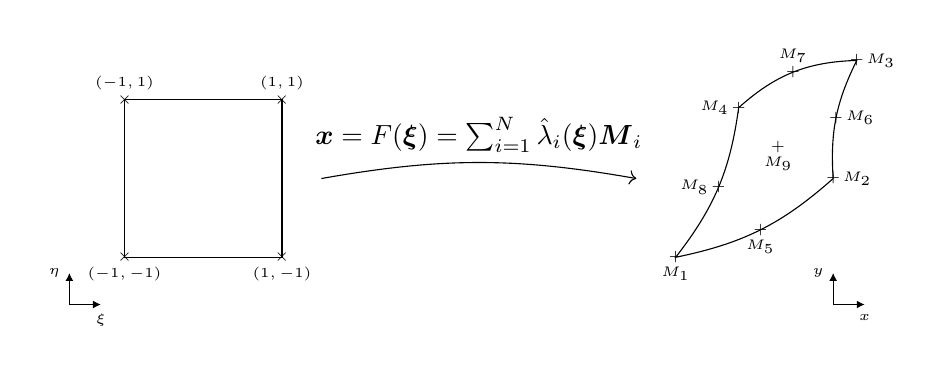
\begin{tikzpicture}[background fill=white]
    % Background rectangle
    % \fill[color=red] (-1,-1) rectangle (10,3);

    % Globals
    \pgfmathsetmacro{\refXMin}{0}
    \pgfmathsetmacro{\refXMax}{2}

    % Ref quad
    \coordinate (REF_SW) at (\refXMin, \refXMin);
    \coordinate (REF_NE) at (\refXMax, \refXMax);
    \draw[color=black] (REF_SW) rectangle (REF_NE);

    \pgfmathsetmacro{\x}{\refXMin};
    \pgfmathsetmacro{\y}{0};
    \coordinate (A) at (\x,\y);
    \node[font=\tiny] at (A) {$\times$};
    \node[below, font=\tiny] at (A) {$(-1,-1)$};

    \pgfmathsetmacro{\x}{\refXMax};
    \pgfmathsetmacro{\y}{0};
    \coordinate (B) at (\x,\y);
    \node[font=\tiny] at (B) {$\times$};
    \node[below, font=\tiny] at (B) {$(1,-1)$};

    \pgfmathsetmacro{\x}{\refXMax};
    \pgfmathsetmacro{\y}{\refXMax};
    \coordinate (C) at (\x,\y);
    \node[font=\tiny] at (C) {$\times$};
    \node[above, font=\tiny] at (C) {$(1,1)$};

    \pgfmathsetmacro{\x}{\refXMin};
    \pgfmathsetmacro{\y}{\refXMax};
    \coordinate (D) at (\x,\y);
    \node[font=\tiny] at (D) {$\times$};
    \node[above, font=\tiny] at (D) {$(-1,1)$};

    \pgfmathsetmacro{\x}{\refXMin - 0.7}
    \pgfmathsetmacro{\y}{\refXMin - 0.6}
    \draw[-{Latex[length=1mm, width=1mm]}] (\x,\y) -- ++(0.4, 0) node[below] {\tiny $\xi$};
    \draw[-{Latex[length=1mm, width=1mm]}] (\x,\y) -- ++(0, 0.4) node[left] {\tiny $\eta$};


    % Map line
    \pgfmathsetmacro{\arrowWidth}{4}
    \pgfmathsetmacro{\arrowMarginX}{0.5}
    \pgfmathsetmacro{\x}{\refXMax+\arrowMarginX}
    \pgfmathsetmacro{\y}{(\refXMax-\refXMin)/2}
    \coordinate (LINE_W) at (\x, \y);
    \pgfmathsetmacro{\x}{\x+\arrowWidth}
    \coordinate (LINE_E) at (\x, \y);
    \draw[->] (LINE_W) to[bend left = 10] node[midway, above]{
        $\bo{x} = F(\bo{\xi}) = \sum_{i=1}^N \hat{\lambda}_i(\bo{\xi})\bo{M}_i$
    } (LINE_E);

    % Physical quad
    \pgfmathsetmacro{\x}{\refXMax + 2*\arrowMarginX + \arrowWidth};
    \pgfmathsetmacro{\y}{0};
    \coordinate (A) at (\x,\y);
    \node[font=\tiny] at (A) {+};
    \node[below, font=\tiny] at (A) {$M_1$};

    \pgfmathsetmacro{\x}{\x + 2};
    \pgfmathsetmacro{\y}{\y + 1};
    \coordinate (B) at (\x,\y);
    \node[font=\tiny] at (B) {+};
    \node[right, font=\tiny] at (B) {$M_2$};

    \pgfmathsetmacro{\x}{\x + 0.3};
    \pgfmathsetmacro{\y}{\y + 1.5};
    \coordinate (C) at (\x,\y);
    \node[font=\tiny] at (C) {+};
    \node[right, font=\tiny] at (C) {$M_3$};

    \pgfmathsetmacro{\x}{\x - 1.5};
    \pgfmathsetmacro{\y}{\y - 0.6};
    \coordinate (D) at (\x,\y);
    \node[font=\tiny] at (D) {+};
    \node[left, font=\tiny] at (D) {$M_4$};

    \pgfmathsetmacro{\x}{\x + 0.5};
    \pgfmathsetmacro{\y}{\y - 0.5};
    \coordinate (E) at (\x,\y);
    \node[font=\tiny] at (E) {+};
    \node[below, font=\tiny] at (E) {$M_9$};

    \draw[font=\tiny] (A) to[bend right = 15] node[midway] {+} node[midway,below] {$M_{5}$} (B) to[bend left = 15] node[midway] {+} node[midway,right] {$M_{6}$} (C) to[bend right = 20] node[midway] {+} node[midway,above] {$M_{7}$} (D) to[bend left=15] node[midway] {+} node[midway,left] {$M_{8}$} cycle;

    \pgfmathsetmacro{\x}{\refXMax + 2*\arrowMarginX + \arrowWidth + 2}
    \pgfmathsetmacro{\y}{0 - 0.6}
    \draw[-{Latex[length=1mm, width=1mm]}] (\x,\y) -- ++(0.4, 0) node[below] {\tiny $x$};
    \draw[-{Latex[length=1mm, width=1mm]}] (\x,\y) -- ++(0, 0.4) node[left] {\tiny $y$};

\end{tikzpicture}
\end{document}